\documentclass[../summary.tex]{subfiles}

\begin{document}
	
	\section{Biodiversity}
	
	\subsection{Study guide}
	
	Module 2 (Biodiversity) sketches basic insights biodiversity, different types of diversity, in an historical perspective and with options for the future. Make sure to understand:
	\begin{itemize}
		\item The different types of diversity
		\item Historical evolution of biodiversity
		\item The importance of biodiversity
		\item How can biodiversity be measured and challenges in this?
		\item The important treats for biodiversity
		\item Different options to restore biodiversity
		\item Being able to interpret data with regard to biodiversity
	\end{itemize} 
	
	Don’t learn the specific examples by heart, do not learn specific vocabulary by heart (such as Cambrian or Cretaceous).
	\\
	
	\subsection{Types of diversity}
	The variability among living organisms from all sources, including, inter alia, terrestrial, marine and other aquatic ecosystems and the ecological complexes of which they are parts. This includes the diversity within species, between species and of ecosystems
	\\
	\\
	The first type of biodiversity is \textbf{genetic diversity} or diversity within species. It is the amount of naturally occurring genetic variation among individuals of the same species. 
	\\
	\\
	Another type of diversity is \textbf{species diversity}. This type is often defined as the number of species at a certain location. Figure \ref{fig:diversity_species} gives an indication of this diversity.
	\\
	\\
	Thirdly, there also is \textbf{diversity in ecosystems}. There are a lot of different ecosystems around the globe: from the boreal forest at high latitudes to tropical forests around the equator, but also aquatic ecosystems like lake systems, coral reefs and mangroves count towards ecosystem diversity.
	\\
	\begin{figure}[htbp]
		\centering
		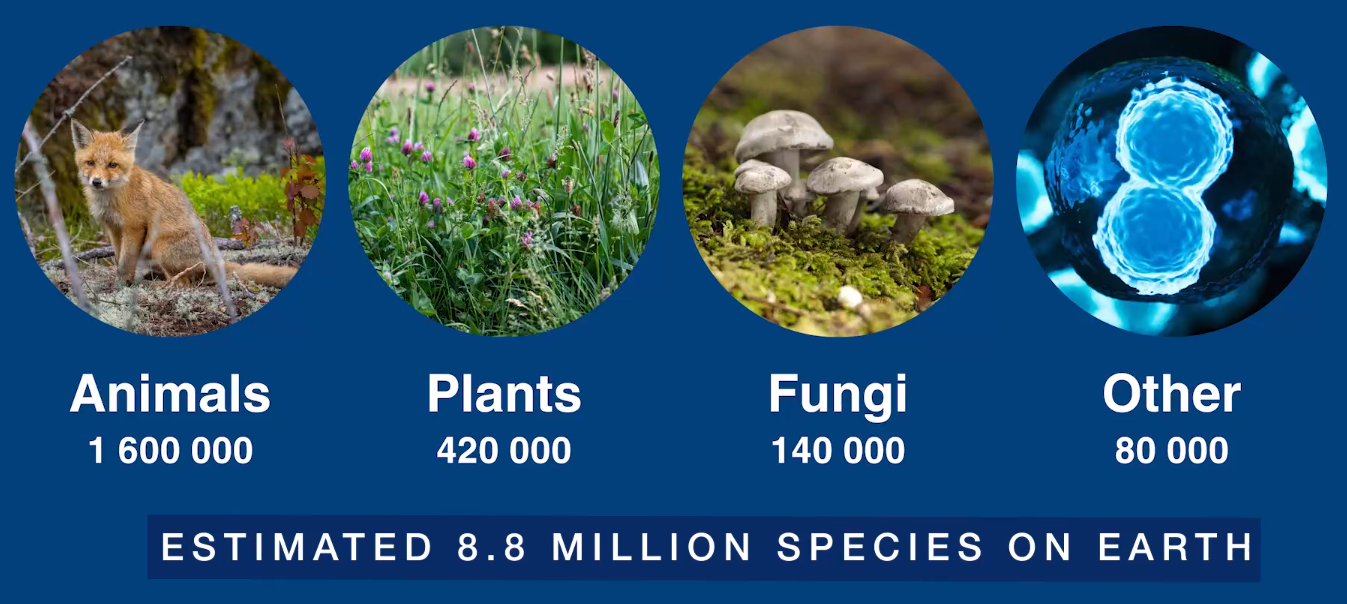
\includegraphics[width=0.75\linewidth]{images/2-diversity_species.png}
		\caption{Diversity in species}
		\label{fig:diversity_species}
	\end{figure}
	
	\subsection{Historical evolution of biodiversity}
	Biodiversity first started to get highly impacted when the Homo sapiens left the African continent to colonize the rest of the globe around 50.000 years ago. Modern humans colonized the globe in four different waves. A first one from Africa to SE Asia and Australia about 50.000 before present, a second one to Europe and central Asia (20 to 30 thousand years BP), a third one through the Americas, and a recent final wave, with the colonization of more remote oceanic island such as Hawaii, Madagascar and New Zealand, less than 1000 years ago.This colonization was paired with a major extinction wave among the megafauna. The biggest reason for this extinction is hunting. 
	\\
	\\
	This extinction of species is still ongoing. Since 1500 there are about 160 known extinct bird species, 60 extinct mammal species and 199 species of other vertebrate groups. Even today, there still are a lot of species threatened with extinction. 
	
	\subsection{The importance of biodiversity}
	In the Ecosystem Services cascade of Figure \ref{fig:ecosystems_services_cascade}, we see the integrated social-ecological system with to the left the ecosystem and to the right the human society. The ecosystem has its composition, structure and function, which all are determined by its biodiversity. The human society receives a flow of ecosystem services from the ecosystem, which contribute to the prosperity and well-being of its members. 
	\\
	\\
	Ecosystem Services are the goods and services humans get from ecosystems and can be divided in three main categories: provisioning, regulating and cultural services. The \textbf{provisioning services} consist of the material flows, like agricultural crops for food, wood for construction, biomass for energy or drinking water. \textbf{Regulating services} are those that provide environmental protection like erosion control, air cooling and filtering by vegetation or climate mitigation through carbon uptake and storage in forests, peatlands and soils. \textbf{Cultural services} include the diverse spiritual, recreational and scientific experiences ecosystems provide to humans. All these services directly depend on biodiversity.
	\begin{figure}[htbp]
		\centering
		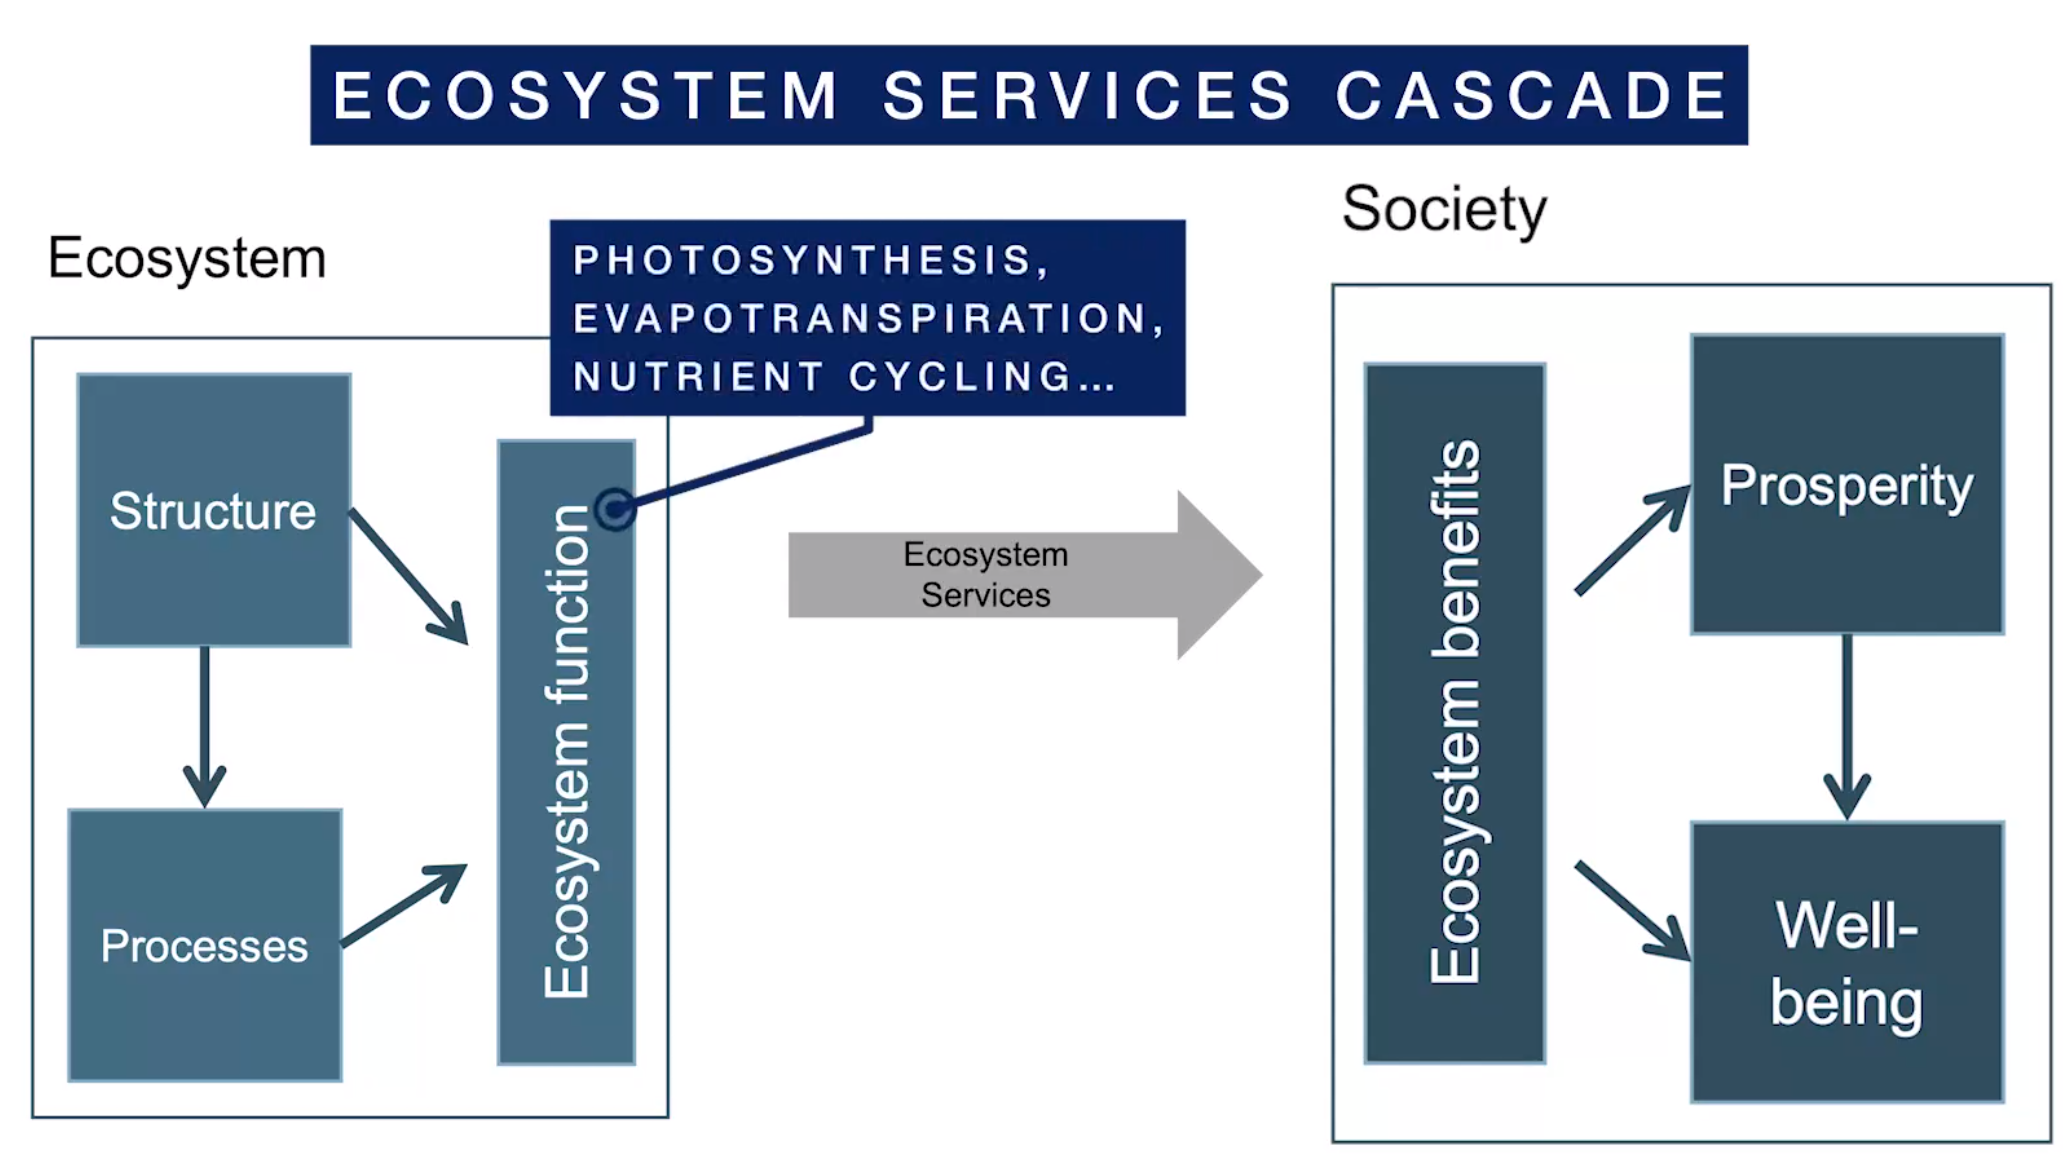
\includegraphics[width=1\linewidth]{images/2-ecosystem-services-cascade.png}
		\caption{Ecosystem Services cascade}
		\label{fig:ecosystems_services_cascade}
	\end{figure}
	\newpage
	There is a \textbf{positive but asymptotic} biodiversity – ecosystem service relationship. This relationship is visualised in Figure \ref{fig:relationship_biodiversity_ecosystems_services}. This means that increasing biodiversity leads to an increase in ecosystem service performance up to a certain extent, after which adding more biodiversity does not much further increase the service provision. It also means that losing some biodiversity as a consequence of human ecosystem degradation may not directly lead to large losses in ecosystem services, but that a further degradation over a critical threshold of species loss will lead to strong reductions in ecosystem services.
	\begin{figure}[htbp]
		\centering
		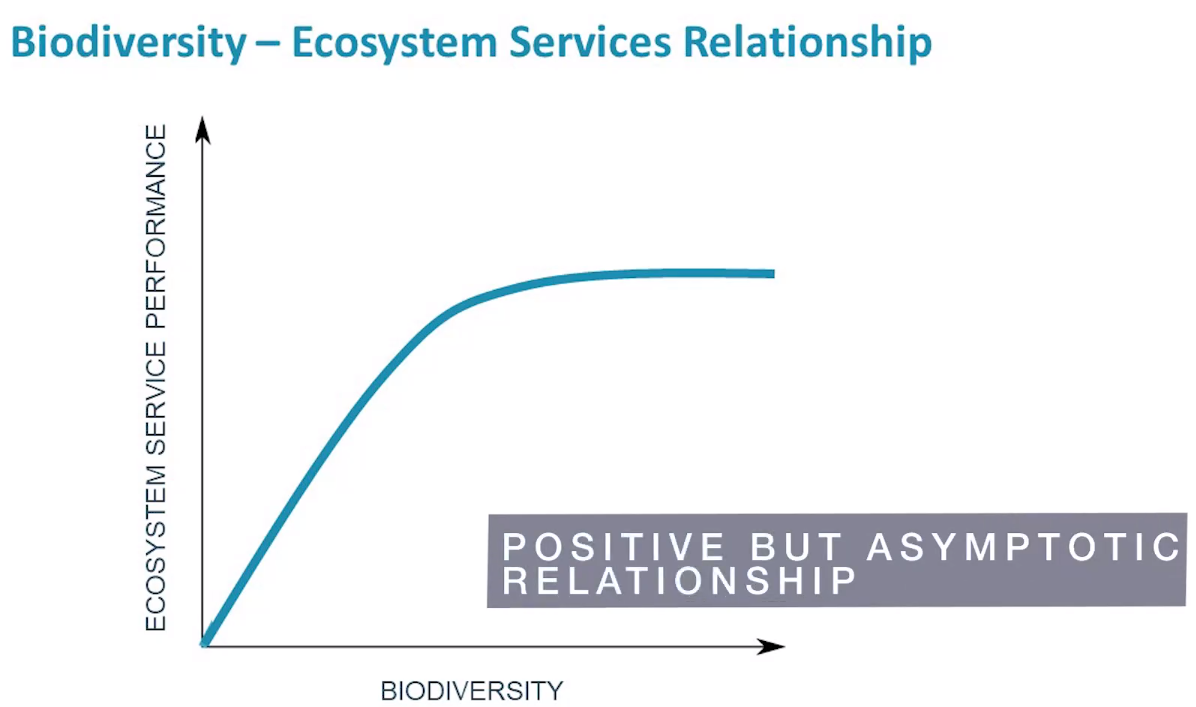
\includegraphics[width=1\linewidth]{images/2-biodiversity-ecosystem-services-relationship.png}
		\caption{Relationship between biodiversity and ecosystems services}
		\label{fig:relationship_biodiversity_ecosystems_services}
	\end{figure} 
	
	\subsection{Measuring of biodiversity}
	To directly measure the effect of a human intervention on the level of biodiversity, we require evidence of a clear causal relationship between intervention and impact, the absence of other confounding factors and clear decisions on which elements of biodiversity are considered. Hence, measuring and monitoring biodiversity is very complex. For this reason often simplified proxies for biodiversity are used, e.g. indicator species, which are known to be sensitive for certain human-induced disturbances, or multi-taxa approaches, to sense the impact on different groups of organisms. Measuring the different dimensions of biodiversity requires a combination of different techniques from satellites to camera traps or citizen science. 
	\\
	\\
	In order to create some structure in this multitude of information, the international community (GEO-BON) developed a framework of Essential Biodiversity Variables (EBV) including the following classes: genetic composition, species populations,  species traits, community composition, ecosystem structure and ecosystem functioning.
	\\
	\\
	Monitoring species population is today the most common indicator method. Observations from experts and citizen science are brought together in the GBIF global biodiversity database. This data together with other data sources are used to build and update IUCN Red List as the major indicator tool for global biodiversity loss.
	\\
	\\
	A very different approach is to measure so-called mid-point indicators. They do not measure the biodiversity loss itself, but rather quantify the frequency and intensity of the damaging interventions. These indicators assume a known relationship between intervention and effect, which is a rather rough approach. Their advantage is that they are much cheaper and have much better data availability than measuring biodiversity effects itself. Examples are area impacted by irrigation, fertilization, biocide use,… .
	
	\subsection{Treats for biodiversity} 
	The main threats to biodiversity can be categorized in 5 different drivers, referred to as the evil quintet. In decreasing order of importance these are habitat loss, overexploitation through hunting and fishing, climate change, pollution and invasive species. Apart from these threats there are other threats that do not fit clearly into these categories, such as for example wildfire or direct human disturbances due to recreational activities.
	\\
	\\
	\textbf{Habitat loss} refers to the transformation of natural habitats into other land uses. It is mainly caused by expanding agricultural land which is especially problematic in the tropics and subtropics.
	\\
	\\
	\textbf{Overexploitation} through hunting and fishing is the second most important threat. It can happen for food or for valued body parts such as ivory.
	\\
	\\
	\textbf{Climate change} is a newly emerging threat to biodiversity. The climate can become too hot or too dry for a species to persist. And very often northward migration of the species to a more mild climate is hampered through habitat loss.
	\\
	\\
	\textbf{Pollution} mainly refers to the effects of agrochemicals such as pesticides and the effects of overuse of fertilizers.
	\\
	\\
	\textbf{Invasive species} may outcompete or predate the indigenous species. They can also introduce new diseases and pests.

	\subsection{Restoring biodiversity}
	There are a couple ways we can try to conserve and restore biodiversity. The first model we will cover is the land sparing-sharing model. \textbf{Land sharing} or nature friendly farming (left on Figure \ref{fig:land-sharing-sparing}) involves integrating practices which benefit biodiversity within the area producing the food. There is however a limit to how friendly one can make farmland for wild species without reducing the yields too much, and lower yields mean that more land is needed to produce each ton of food, making it harder to create more space for nature.
	\\
	\\
	\textbf{Land sparing} on the other hand (right on Figure \ref{fig:land-sharing-sparing}) starts from the observation that high-yielding agriculture can reduce the area needed to meet a given level of demand for food. Land sparing will concentrate higher-yielding production in some parts of the landscape while simultaneously retaining or restoring other parts of the landscape for nature.
	\\
	\\
	When studying this model, the key finding is that most species would have larger populations if a given amount of food is produced on as small an area as possible, while sparing as large an area of native vegetation as possible. 
	\\
	\begin{figure}[htbp]
		\centering
		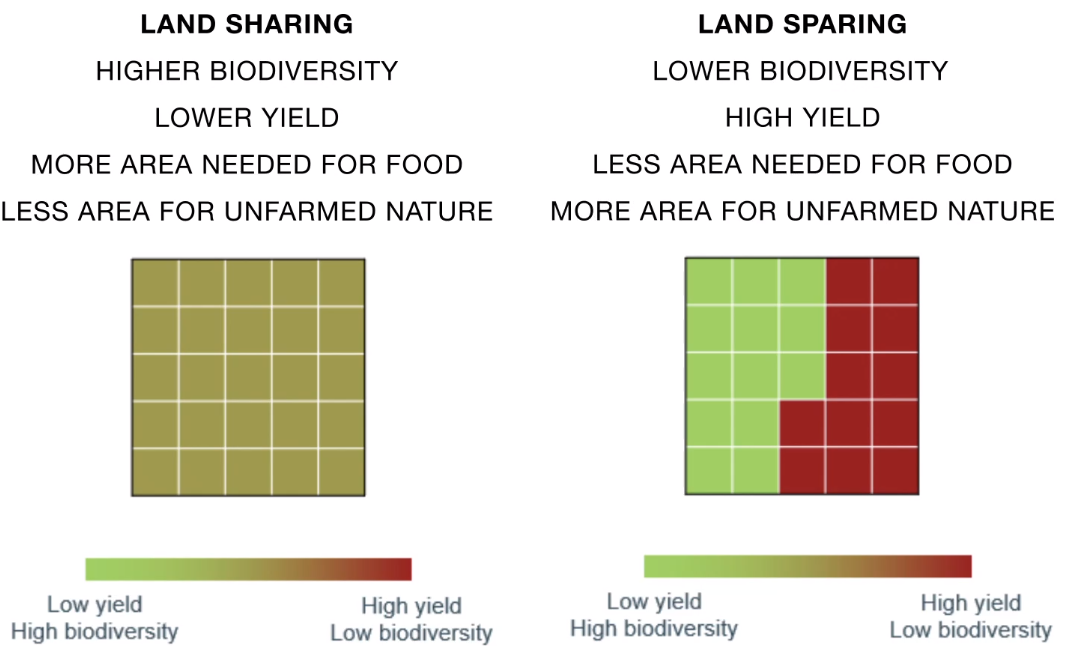
\includegraphics[width=1\linewidth]{images/2-land-sharing-sparing.png}
		\caption{Land sharing versus land sparing}
		\label{fig:land-sharing-sparing}
	\end{figure}
	\newpage
	A second subject we can study, is human activity. \textbf{Ecological restoration} is the process of assisting the recovery of damaged, degraded, or destroyed ecosystems. Restoration aims to reverse damage and protect the biodiversity and services that ecosystems provide.
	\\
	\\
	Recently, \textbf{rewilding} has emerged as a new approach to ecosystem restoration. It promotes "wild, autonomous" nature, with natural processes driven by keystone species and abiotic processes leading the way instead of human intervention. Some examples of common approaches employed in rewilding initiatives are the reintroduction of large fauna species or trophic rewilding, restoring habitat connectivity, wetland restoration and natural regeneration and succession. 
	
\end{document}